\chapter{Editing}
There are three types of objects which can be exported: Empties,
Meshes and Lamps. Other objects like curves and surfaces will have to be
converted to meshes before attempting to export them.

\begin{propertyBlender}{Location}
    Blender's location property. The engine will round it down to three decimal places.
\end{propertyBlender} 

\begin{propertyBlender}{Scale}
    Blender's scale property cannot be exported directly as the engine 
    only supports uniform scale. If a non-uniform scale value is used the export 
    script will try to apply the scaling factor to the object and it's children.
    However this is not entirely reliable and may cause issues especially with 
    animations. Therefore it is recommended to either keep the scale uniform or 
    apply it manually before exporting.
\end{propertyBlender}  

\begin{propertyAurora}{Wirecolor}
    This property is present for all object, but unused by the engine. It can safely be ignored 
    and exists only for compatibility reasons.
\end{propertyAurora}


\section{Empties}
Empties are used to group objects and indicate special 
locations. Empties are called Dummies in MDL files.


\subsection{Aurora Root}
Each MDL requires at least one Empty: The Aurora Root or Rootdummy. It holds 
additional information and indicates which objects belong to an MDL. All children
of a single Rootdummy are considered to be part of the same MDL. \\

Any Empty without a parent is automatically considered a Rootdummy. 
The Rootdummy must have the same name as the MDL file (minus the file extension). 
A Rootdummy has the following properties:

\begin{propertyAurora}{Classification}
Determines the type of MDL
\begin{description}[leftmargin=6em,style=nextline]
    \item[Item] Any inventory item.
    \item[GUI] Unknown.
    \item[Effect] For visual effects.
    \item[Door] Doors, be it generic or for tilesets.
    \item[Character] Creature or placeables. 
    \item[Tile] For tilesets.
    \item[Unknown] Avoid using this. It may be set during import.
\end{description}
\end{propertyAurora}

\begin{propertyAurora}{Supermodel}
Reference to another model. When a model is assigned a supermodel, 
the engine loads the animation data from the supermodel on to the 
pieces that have the same name in the current model.
\end{propertyAurora}

\begin{propertyAurora}{Animationscale}
Used in conjunction with the supermodel. This property scales the current model in relation to 
its supermodel, i.e. a value of 0.5 means the current model is half the size of the supermodel.
\end{propertyAurora}

\subsection{Dummy}
Simple Empties with a parent are either used to group objects or
indicate a special location to the engine. \\

\begin{figure}
  \centering
  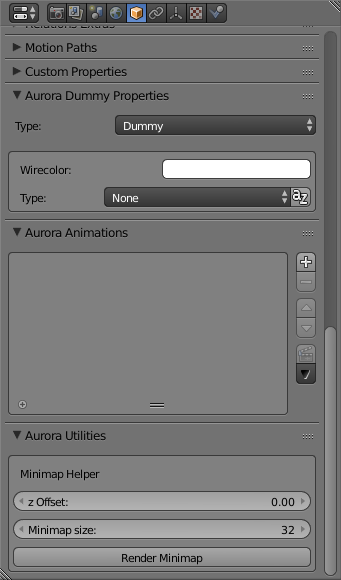
\includegraphics[trim=0 0 0 0, clip, width=0.33\textwidth]{panel_dummy}
  %\caption[panel dummy]{Dummy Property Panel}
  \label{fig:panel_dummy}
\end{figure}

\begin{propertyAurora}{Dummytype}
The following types of Dummies are available:
\begin{description}[leftmargin=6em,style=nextline]
    \item[None] Simple dummy without any special purpose.
    \item[Ground] Indicates the ground level for spells/ visual effects
    \item[Impact] Impact target for most spells/ visual effects.
    \item[Head Hit] Spells/ visual effects
    \item[Head] Head location for Spells/ visual effects
    \item[Hand] Point of origin for (some) spells. If a spell/ visual is originating from this mdl, this will be the point of origin most of the time.
    \item[Use 1] Use Node for placeables or doors. Upon receiving a use command a character will move to the closest of the two use nodes.
    \item[Use 2] Use Node for placeables or doors. Upon receiving a use command a character will move to the closest of the two use nodes.
\end{description}
\end{propertyAurora}
None of the special Dummies are mandatory. If one is
missing from the MDL, the engine will use (0,0,0) as the default location
for that particular Dummy. \\

Selecting the type is not enough to make a Dummy work, they need to have
the correct name or to be precise: The correct suffix.
The export script will try to generate a valid name depending on
the Dummy's type, but it is recommended to do it manually to avoid naming
conflicts. \\

Use the button next to the Dummytype selector to generate a
working name. The Rootdummy's name will be used to create a working
suffix for the selected Dummytype. \\

\subsection{Reference Node}
The purpose and usage of these nodes is unknown. Supposedly it can be used to
reference other MDL files. These nodes can be found in some visual effects and reference fx\_ref 
most of the time.

\begin{propertyAurora}{Reference Model}
The name of another MDL file without file-extension.
\end{propertyAurora}

\begin{propertyAurora}{Reattachable}
Unknown purpose.
\end{propertyAurora}

\subsection{Patch Node}
The purpose and usage of these nodes is unknown. They occur in some visual effects, but
they seem to behave exactly like normal dummy nodes, i.e they have the same
attributes.

\section{Meshes}

\subsection{Trimeshes}

\begin{figure}
    \centering
    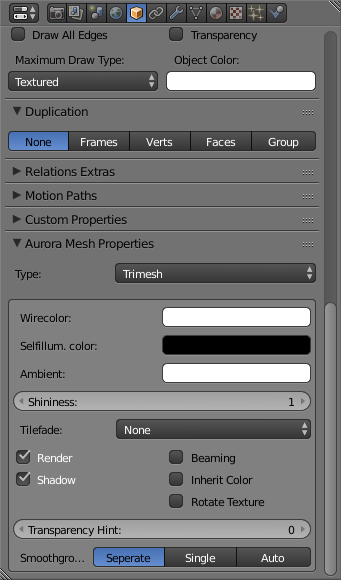
\includegraphics[trim=0 0 0 0, clip, width=0.33\textwidth]{panel_trimesh}
    %\caption[panel trimesh]{Trimesh Property Panel}
    \label{fig:panel_trimesh}
\end{figure}

Any newly created mesh object is considered a trimesh by default. As the name 
suggests it consists of triangles, but it is not necessary to explicitly 
convert the faces to triangles as Neverblender does that automatically 
during the export process.

\begin{figure}
    \centering
    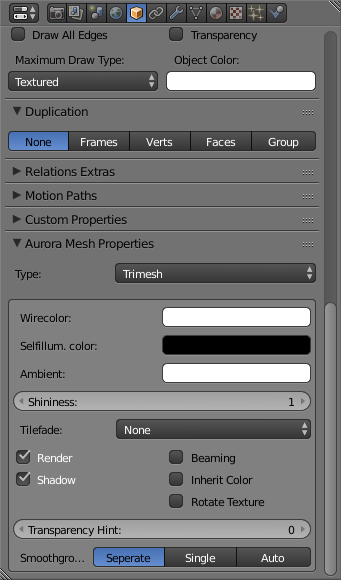
\includegraphics[trim=0 0 0 0, clip, width=0.33\textwidth]{panel_trimesh}
    %\caption[panel_trimesh]{Trimesh Property Panel}
    \label{fig:panel_trimesh}
\end{figure}

\begin{propertyAurora}{Self-Illumination Color}
Makes the mesh glow without acting as a light source.
This property will not be visible in Blender.
\end{propertyAurora}

\begin{propertyAurora}{Ambient Color}
OpenGL material property. The engine uses per-object ambient light whereas Blender's 
defines it on a per scene basis. Therefore this property will not be visible in Blender.
\end{propertyAurora}

\begin{propertyAurora}{Shininess}
Shininess requires a matching texture information file (*.txi).
\end{propertyAurora}

\begin{propertyAurora}{Tilefade}
This property is only relevant for tiles. It controls whether this 
mesh will turn invisible to offer a clear line of sight on the character.
\begin{description}[leftmargin=6em,style=nextline]
    \item[None] This mesh will always be visible.
    \item[Fade] The object will fade.
    \item[Base] Unknown
    \item[Neighbor] The object will fade along with meshes in neighboring tiles.
\end{description}
\end{propertyAurora}

\begin{propertyAurora}{Render}
Controls whether this object will be rendered. The geometry will still be loaded to the memory and 
casts shadows, even if this is unchecked. This is frequently used in conjunction with the Shadow
property to create a shadow volume object which is simpler than the actual visible geometry.
\end{propertyAurora}

\begin{propertyAurora}{Shadow}
Controls whether this objects should cast a shadow. It is recommended to 
disable Shadows for complex meshes with a large amount of triangles and create 
a lower poly mesh with disabled rendering and enabled shadows.

Failing to do so might negatively impact performance or result in corrupt shadows as 
the engine is only capable of handling shadows for simple, convex objects.
\end{propertyAurora}

\begin{propertyAurora}{Beaming}
For light-rays. This is how the light-rays in the forest tileset are generated. 
Light rays cannot be made specifically for a tile, as tiles can rotate.
Instead a different kind of shadow was created where the shadow
volume is rendered at an alpha value and a specific colour. To create shadow
volumes, make a group of simple triangles above the camera level and enable
this flag.
\end{propertyAurora}

\begin{propertyAurora}{Inherit Color}
Unused. It was originally intended for tint-able objects to be 
able to inherit their parent's color.
\end{propertyAurora}

\begin{propertyAurora}{Rotatetexture}
This is for ground mapping on tilesets. When a model with
this flag is rotated, the engine knows to rotate the uv coordinates back 
to the original position. This eliminates texture seams on floors 
and grass over tile edges.
\end{propertyAurora}

\begin{propertyAurora}{Transparencyhint}
As transparency can be extremely costly to calculate from alpha values on a
texture, this property gives the engine priority values on transparent objects to let it
know which are more important. If an object has a transparency hint of 1, then it
will be rendered after a transparent object that has a value of 0. This does not work 
on dynamic objects, it only affects static objects.
\end{propertyAurora}

\begin{propertyAurora}{Smoothgroup}
Controls smoothing groups or shading groups are created
\begin{description}[leftmargin=6em,style=nextline]
    \item[Separate] Each face will have its own smoothing group. This results in no smoothing at all.
    \item[Single] All faces belong to a single smoothing group. Meshes will be smoothed completely.
    \item[Auto] Auto generate smoothing groups, depending on the settings in blender and edges marked as sharp. Replicates blenders smoothing as closely as possible.
\end{description}
\end{propertyAurora}

\subsection{Danglymeshes}

\begin{figure}
    \centering
    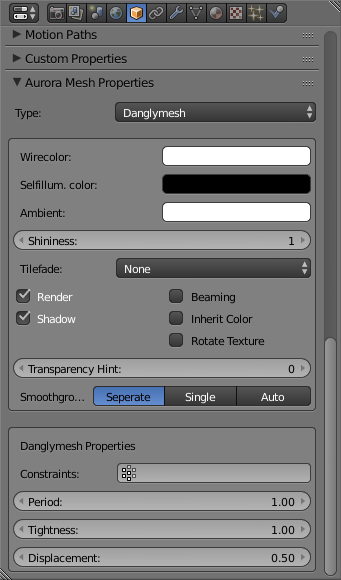
\includegraphics[trim=0 0 0 0, clip, width=0.33\textwidth]{panel_danglymesh}
    %\caption[panel danglymesh]{Danglymesh Property Panel}
    \label{fig:panel_danglymesh}
\end{figure}

Danglymeshes are Trimeshes which are "bouncy" or "dangly". They are affected by
wind, character movement and visual effects. Danglymeshes possess the same 
properties as Trimeshes in addition to the following ones.

\begin{propertyAurora}{Dangle group} 
The dangle group is a vertex group containing the weights of vertices for the danglymesh. 
You must select an existing vertex group. Vertex paint may be used to paint the weights. A vertex with a weight of
0.0 will not change position.
\end{propertyAurora}

\begin{propertyAurora}{Period} 
Determines how quickly the vertices move and how fast they come to a rest.
\end{propertyAurora}
\begin{propertyAurora}{Tightness} 
The 'tension' in the object, restricting movement. 
\end{propertyAurora}
\begin{propertyAurora}{Displacement} 
Determine show far the vertices are allowed to move. This is further restricted by the Dangle group.
\end{propertyAurora}


\subsection{Skinmeshes}
A skinmesh is used to create skeletal animations. At the moment it is not 
possible to use Blender's armature system directly. Instead several vertex groups 
must be created with their names matching one of the other trimeshes in the MDL. 
Unfortunately this means that no animations are visible in blender which makes
creation of new skinmeshes difficult.


\subsection{Animmeshes}
Animeshes are Trimeshes with animated UV coordinates or vertices, the latter requires the use of a 
shape key. The AnimAll Add-On is required to animate UV coordinates and shape keys. The number of 
animated keyframes for Animmeshes is limited to two (start and beginning of the animation).

\begin{propertyAurora}{Shapekey} 
    The shape key from which the animation data is taken. If no key is specified, vertex animations will
    not be exported.
\end{propertyAurora}

\subsection{Walkmeshes}
Walkmeshes indicate where a character can walk. It is necessary to select 
the appropriate type of walkmesh, which depends on the type of model itself. 

\begin{propertyAurora}{Walkmeshtype} 
Sets the type of a walkmesh. The available types depends on the classification of the MDL:
\begin{description}[leftmargin=10em,style=nextline]
    \item[Tileset] Walkmesh for tiles. This will also affect footstep sounds and grass growth. No overlapping faces are allowed. To specify the surface type, it is necessary to add the walkmesh materials to the object. You can add all walkmesh materials by clicking on the {\textit{Load walkmesh materials}} Button in the Aurora mesh properties panel. The materials are then added as materials slots and accessible through the materials tab in the object properties.
    The export script will create a matching {\textit{.wok}} file. 
    \item[Door: Closed] The walkmesh for the closed state of a door. Blocks movement.
    \item[Door: Open 1] The Walkmesh for the first open state of a door. Blocks movement.
    \item[Door: Open 2] The Walkmesh for the second open state of a door. Blocks movement.
    \item[Placeable] Walkmesh for placeables. Blocks movement.
\end{description}
\end{propertyAurora}

\section{Emitters}
Support for Emitters is rudimentary. Blenders particle systems is too
different to allow a direct import, instead Emitters are imported as plain
text. While all data will be retained, editing is only possible by altering the 
generated text file for each emitter.

\section{Lamps}
Blender's lamp properties for color and distance will be used for exporting a light.

It is recommended to check \textit{Sphere} to better replicate the resulting effect 
of a light source.

\begin{propertyAurora}{Light type}
There are some special light types, all of which are used to give builders
the ability to select light color in the Toolset.
\begin{description}[leftmargin=8em,style=nextline]
    \item[Mainlight 1] For Tiles only. The Lamp Color property will not affect this lamp as it can be changed in the Toolset.
    \item[Mainlight 2] For Tiles only. The Lamp Color property will not affect this lamp as it can be changed in the Toolset.
    \item[Sourcelight 1] For Tiles only. This is actually a burning flame. Color can be changed in the Toolset.
    \item[Sourcelight 2] For Tiles only. This is actually a burning flame. Color can be changed in the Toolset.
    \item[Default] Default type, can always be used. Blenders lamp properties will be used (color and distance)
\end{description}
\end{propertyAurora}

\begin{propertyAurora}{Priority}
Use by the engine's light manager to prevent using too many lights that affect dynamic 
objects. This relates to the light count setting in the game. In order for the manager 
to know which lights can be culled first, a priority is assigned to each light, ranging from 1-5, 
1 being the highest priority. This is the general scheme:
\begin{enumerate}
    \item The sun \& the moon
    \item Torches \& light spells
    \item Spells, general lights
    \item Un-needed tile lights
    \item Other un-needed lights, for example from weapons.
\end{enumerate}
\end{propertyAurora}

\begin{propertyAurora}{Ambient Only}
This controls if the light is only an ambient light source or
if it is directional as well.
\end{propertyAurora}

\begin{propertyAurora}{Fading}
When a light is loaded or dropped from a scene, the light will 'flick' on and off. 
If this check is on, the light will take a moment to fade on or off for a better overall feel.
In some cases it’s best to have this un-checked, for things like spells where you want 
the light to be at it’s brightest as soon as it appears.
\end{propertyAurora}

\begin{propertyAurora}{Shadows}
Determines if this light is capable of producing shadows.
\end{propertyAurora}

\begin{propertyAurora}{Is Dynamic}
Unknown.
\end{propertyAurora}

\begin{propertyAurora}{Affect Dynamic}
This controls whether this light affects dynamic objects, i.e. characters.
Disabling this will prevent this light from producing shadows with dynamic
objects, but it will in turn improve performance.

This is a less strict version of the \textit{Shadows} setting.
\end{propertyAurora}

\begin{propertyAurora}{Lensflares}
Add a series of lens-flares for this light. Lens-flares are unavailable for 
Mainlights or Sourcelights. The flare radius is global for all flares of 
this light source and is in cm (as opposed to meters in other distance values).
\begin{description}[leftmargin=6em,style=nextline]
    \item[Texture] Texture for this flare
    \item[Colorshift] Unknown. Possibly color difference from the light color.
    \item[Size] Size of the flares. This will scale the texture.
    \item[Position] Distance from the lights origin. Values from -1 to 1.
\end{description}
\end{propertyAurora}

\section{Materials \& Textures}
MDL files support a single material with a single texture. If multiple 
materials or textures are assigned, the export script will choose the currently 
active one or, failing that, the topmost one.

The following properties are exported:
\begin{itemize}
    \item Diffuse
    \item Specular
    \item Alpha values
\end{itemize}

\subsection*{Alpha}
Neverblender can export either material or texture alpha. When both properties are present 
the latter takes precedence. This matches the output in blenders 3D view (with GLSL mode enabled) 
or renderer.

\section{Animations}
Each animation has to be defined by name and start/end frames. Valid names 
are listed in the reference chapter for each type of MDL.

\subsection{Animation Tools}

\begin{description}
\item[Add \& Delete] Add or delete an animation. Note that keyframes will be deleted too.
\item[Move Back] Move the animations and its keyframes to the end of the timeline for easier editing.
\item[Focus] Sets the start and end frames of the time to the currently selected animation.
\item[Clone] Copies an animation and its keyframes. The copy is added to the end of the timeline.
\item[Scale] Scales an animation up or down
\item[Pad \& Crop] Add or remove a specific amount of keyframes at the start or end of an animation.
\end{description}

\subsection{Animation Properties}
The following properties can be animated:
\begin{itemize}
    \item Location
    \item Rotation
    \item Scale (Uniform only)
    \item Material or Texture Alpha
    \item Self-Illumination color
    \item Lamp color
    \item Lamp distance (Light radius)
    \item Texture coordinates (using AnimAll, 2 key limit)
    \item Vertices (using AnimAll, 2 key limit)
\end{itemize}
Additional animation data is stored in the Rootdummy. Deleting the Rootdummy will result in
the loss of this data.

\begin{propertyAurora}{Name}
    Similar to the Supermodel property, however this overrides only a 
    specific selection of nodes instead of all of them.
\end{propertyAurora}

\begin{propertyAurora}{Root}
    Similar to the Supermodel property, however this overrides only a 
    specific selection of nodes instead of all of them.
\end{propertyAurora}

\begin{propertyAurora}{Transition Time}
    This value influences how much mixing occurs with the previous animation in order to 
    fade smoothly into the current animation. Most animations use the default value of 0.25.
\end{propertyAurora}

\begin{propertyAurora}{Start}
    The animations first frame
\end{propertyAurora}

\begin{propertyAurora}{End}
    The animations last frame
\end{propertyAurora}

\begin{propertyAurora}{Emitter Data}
    Emitter data or other incompatible data will be imported as plain text and saved in a text object. The
    time values are converted to frames during this process.
\end{propertyAurora}

\begin{propertyAurora}{Animation Events}
    Events like footstep sounds. Each event has a name and associated frame
\end{propertyAurora}